\chapter{Unifying Machine Learning and Quantum Mechanics} \label{chp:VMCwRBM}
%\epigraph{Great quote.}{Author}
\iffalse
\begin{figure}[H]
	\centering
	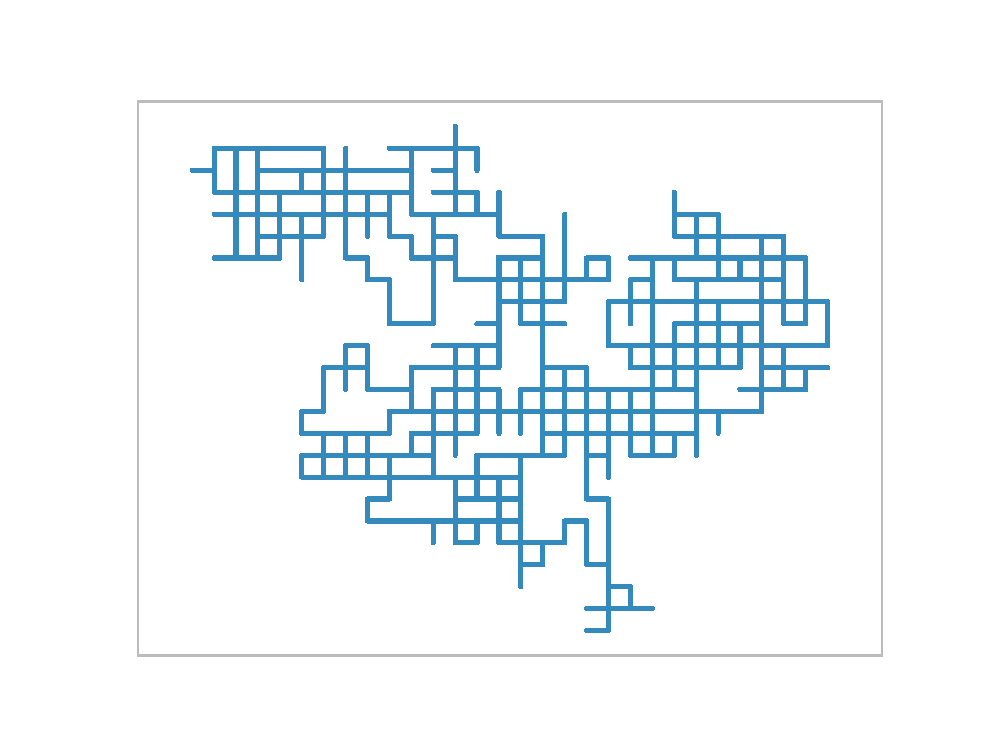
\includegraphics[scale=0.6]{../Images/randomwalk.eps}
	\caption{Random walker on a two-dimensional grid, 1000 moves.}
\end{figure}
\fi

Now as we have introduced the necessary theory, both in the form of quantum theory and machine learning theory, in addition to detailing the variational Monte Carlo (VMC) method, we are ready to unify the machine learning and quantum mechanics. As hinted above, the way we do this is to let a restricted Boltzmann machine define our single-particle functions in the trial wave function, and then just update the function in a normal VMC scheme. This is very similar to the approach of \citet{pfau2019abinitio}, but an essential difference is that they did not restrict the single-particle functions to take the coordinates of a single particle. Further, we investigate how the results change when Jastrow factors with gradually more physical intuition baked in are added. As the main goal is to find a method that requires less physical intuition in order to provide accurate results compared to the traditional methods, adding a simple Jastrow factor is also very interesting. We look at three different cases: a Slater determinant where the single-particle functions are given by a restricted Boltzmann machine (RBM), an RBM with a simple Jastrow added (RBM+SJ) and an RBM with a Padé-Jastrow factor added (RBM+PJ). They are detailed in respective sections below.

\section{Restricted Boltzmann machine without Jastrow factor (RBM)} \label{sec:rbm}
In chapter \ref{chp:methods}, we saw how the VMC method attempts to solve the time-independent Schrödinger equation directly by vary the parameters in a trial wave function. In order to satisfy the anti-symmetry properties of a fermionic many-body wave function, the trial wave function was composed as a Slater determinant,
\begin{equation}
\Psi_T(\bs{R})\propto
\begin{vmatrix}
\phi_1(\boldsymbol{r}_1) & \phi_2(\boldsymbol{r}_1) & \hdots & \phi_N(\boldsymbol{r}_1)\\
\phi_1(\boldsymbol{r}_2) & \phi_2(\boldsymbol{r}_2) & \hdots & \phi_N(\boldsymbol{r}_2)\\
\vdots & \vdots & \ddots & \vdots \\
\phi_1(\boldsymbol{r}_N) & \phi_2(\boldsymbol{r}_N) & \hdots & \phi_N(\boldsymbol{r}_N)
\end{vmatrix}\equiv|\hat{D}(\bs{R})|.
\end{equation}
Even though we want a method which requires as little physical intuition as possible, the wave function needs to obey Fermi-Dirac statistics, and we therefore also approximate the trial wave function with the Slater determinant for the machine learning method. Further, we use the same framework as we did for VMC, but the single-particle functions (SPFs) $\phi_j(\bs{r}_i)$ are given by the marginal distribution of the visible units from a restricted Boltzmann machine, $P(\bs{r})$. For quantum dots, we also add the Hermite polynomials, $H_n(\bs{r})$ to get an unique SPF for each state. We then have
\begin{equation}
\phi_j(\bs{r}_i)=H_j(\bs{r}_i)P(\bs{r}_i)
\end{equation}
where the restricted Boltzmann machine takes all the coordinates as input nodes, i.e., the input vector is $\bs{x}=(x_1, y_1, x_2, y_2, \hdots, x_N, y_N)$ for a two-dimensional system. With this, we end up with a trial wave function that contains more variational parameters than a standard VMC trial wave function, and which hopefully is able to provide a more correct wave function. Further, we will add a simple Jastrow factor to see how this affects the correlations.

\section{RBM with a simple Jastrow factor (RBM+SJ)}
This method, abbreviated RBM+SJ, is just an extension of the RBM method described in the previous section, where we add a simple Jastrow factor to help modeling the electron-electron cusp. When adding a Jastrow factor we also add some more physical intuition to the trial wave function, but the Jastrow factor used here still contains a minimum of physical intuition. It is expressed as
\begin{equation}
J(\bs{R}; \bs{\beta}) = \exp\left(\sum_{i=1}^N\sum_{j>i}^N{\beta_{ij}r_{ij}}\right).
\label{eq:SimpleJastrow}
\end{equation}
where $r_{ij}$ is the radial distance between particle $i$ and $j$ and the $\beta_{ij}$'s are free variational parameters, which are expected to be symmetric since the distance matrix is symmetric. The trial wave function using this method thus takes the form
\begin{equation}
\Psi_T(\bs{R})\propto|\hat{D}_{\uparrow}(\bs{R}_{\uparrow})|\cdot|\hat{D}_{\downarrow}(\bs{R}_{\downarrow})|J(\bs{R};\bs{\beta})
\end{equation}

\section{RBM with a Padé-Jastrow factor (RBM+PJ)}
Lastly, we add the well-known Padé-Jastrow factor to the RBM, abbreviated RBM+PJ, to see how much the results change when a more advanced correlation factor is added. As discussed in section \ref{sec:jastrow}, the Padé-Jastrow factor is constructed to model the electron-electron cusp correctly, and it is also interesting to see how more physical intuition in the trial wave function affects the results. The RBM+PJ trial wave function then reads
\begin{equation}
\Psi_T(\bs{R})\propto|\hat{D}_{\uparrow}(\bs{R}_{\uparrow})|\cdot|\hat{D}_{\downarrow}(\bs{R}_{\downarrow})|J(\bs{R};\beta)
\end{equation}
where we recall that the Padé-Jastrow factor contains the variational parameter $\beta$.